
\documentclass{article}
\usepackage[utf8]{inputenc}
\usepackage{amsmath,amsfonts}
\usepackage{graphicx}

\newtheorem{theorem}{Theorem}[section]
\newtheorem{corollary}{Corollary}[theorem]
\newtheorem{proof}{Proof}[corollary]

\newcommand{\R}{\mathbb{R}}

\title{Report 0: List of Useful Commands}
\author{Zixuan Fan}
\date{09/12/2023}

\begin{document}

\maketitle

\section{Introduction}


Hello World Hello \LaTeX\ ! in this short introduction of the lab report, I will be testing on the mechanics of Latex, starting with the simple formula of $e^{i\pi}+1=0$, and continuing with the formula of:

\begin{align}
\begin{split}
\label{limit}
e&=
\lim_{n\to\infty}
\left(	1+\frac{1}{n}	\right)^n \\
&=\lim_{n\to\infty}	\frac{n}{\sqrt[n]{n!}}.
\end{split}
\end{align}

\noindent The addition of \verb|&| here serves to align the equal sign under the effect of "align"\\

\noindent Note that to begin itemize or enumerate, the first item must follow immediately after

\begin{itemize}
\item Further, let's include the formula of a sum:

$$e=
\sum_{n=0}^{\infty}	\frac{1}{n!},
$$

\item And a continued fraction:

$$e=
2+\frac{1}{1+\frac{1}{2+\frac{2}{3+\frac{3}{4+\frac{4}{5+\ddots}}}}}
$$

\end{itemize}
Equation \ref{limit} can be referenced like this.

\section{More Formulas}

Note that many items here require package amsmath and graphicx in order to function, make sure to import these packages in the beginning of your report.

\begin{enumerate}

\item The format of an integral:

$$\int_a^bf(x)dx$$

\item The format of triple integral:

$$\iiint_0^\infty	f(x)dx
$$

\item The format of single vector:

$$\vec{v}=<v_1, v_2, v_3>$$

\item The format of dot product:

$$\vec{v}\cdot \vec{w}$$

\item The format of matrix:

$$\begin{bmatrix}
1	&	2	&	3 \\
4	&	5	&	6 \\
\end{bmatrix}
$$

\item The format of importing an image:\\
Note that the image must be in the same folder with the report
$$
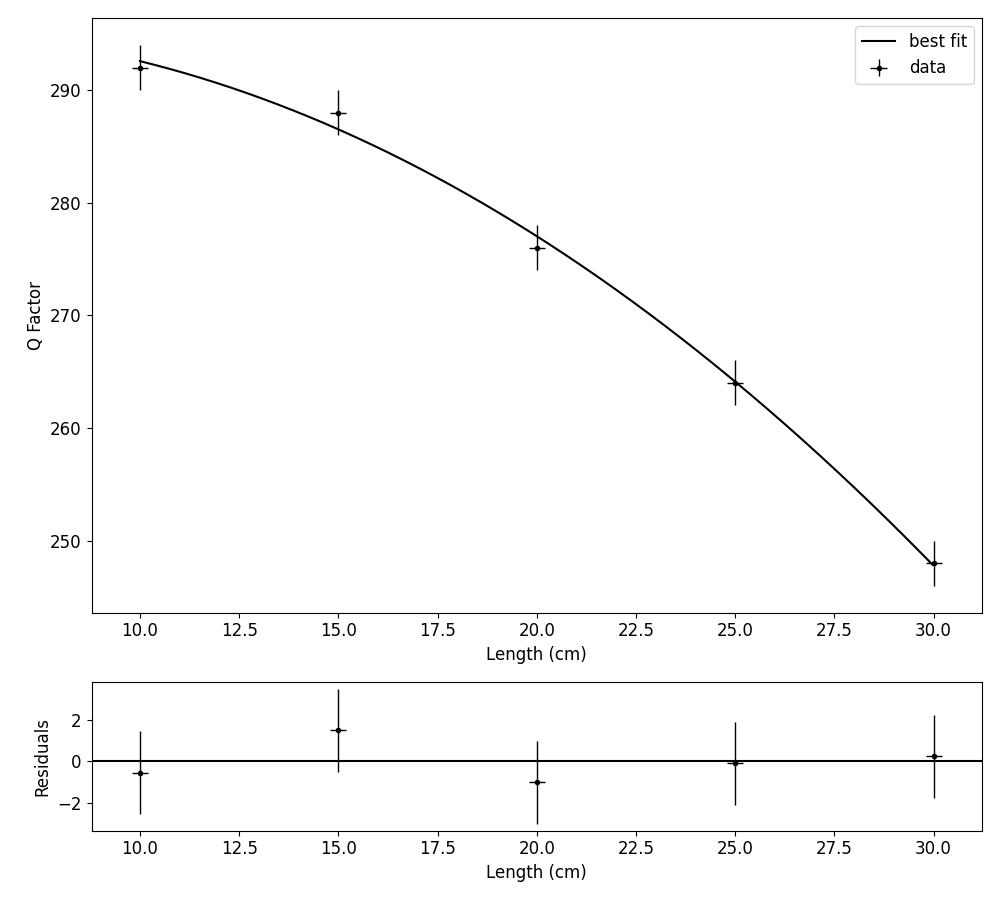
\includegraphics[scale=0.3]{graph.png}
$$

\end{enumerate}


\section{Basic Controls}
This section will cover some of the basic controls that someone using google docs could easily achieve with the click of a button

\begin{enumerate}
\item bold:\\
\textbf{bold characters}

\item italic:\\
\textit{italic characters}

\item underline:\\
\underline{underline characters}

\item Making a table here (Note the h is very important to keep the table right here)

\begin{table}[h]
\caption{A little table}
\label{little table}
\begin{center}
\begin{tabular}{|c|c|c|}
	\hline
	1 & 2 & 3\\\hline
	4 & 5 & 6\\\hline
\end{tabular}
\end{center}
\end{table}

\item I like table \ref{little table} so I will reference it\\ 

\item figures
\begin{figure}[h]
	\centering
	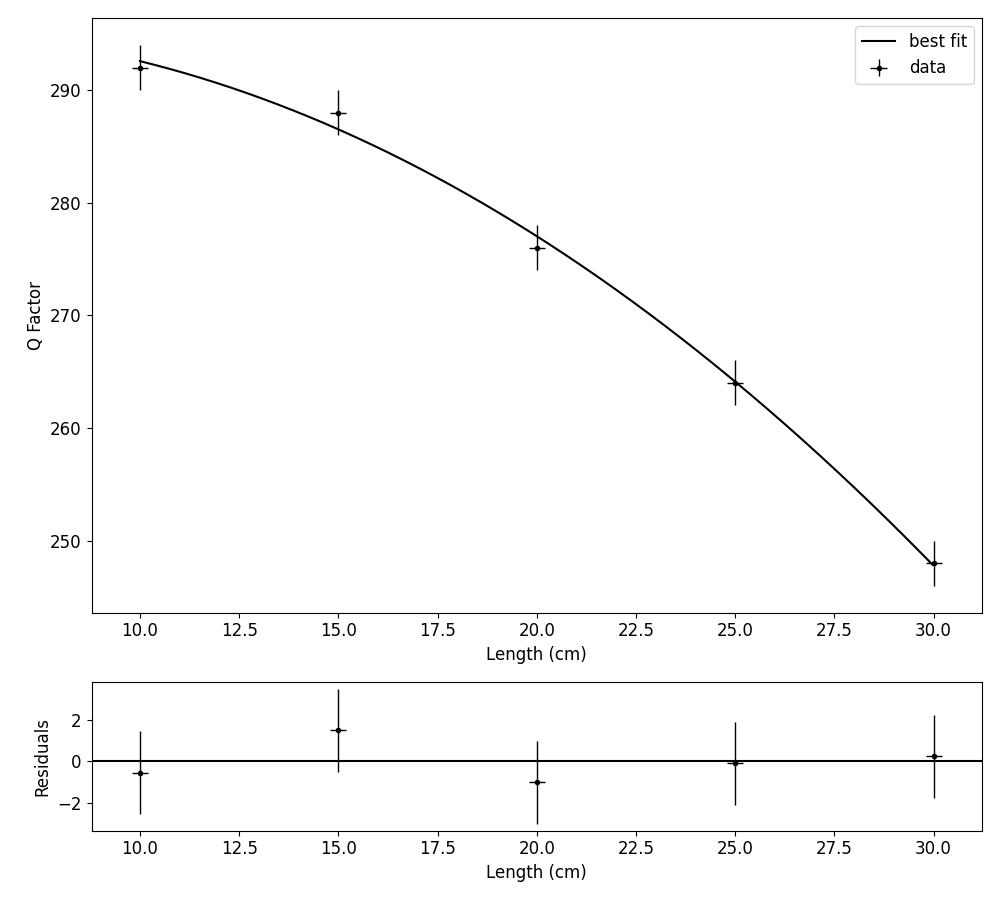
\includegraphics[scale=0.2]{graph.png}
	\caption{A graph}
	\label{fig:myLabel}
\end{figure}

\item inserting theorems, corollaries, and proofs(Note that newtheorem must be thrown in)
\begin{theorem}[test]
This is not a test theorem
\end{theorem}

\begin{corollary}[also a test]
This is not a test corollary
\end{corollary}

\begin{proof}[still a  test]
This is a test proof
\end{proof}

\item Real number set:\\
This is a real number set $\mathbb{R}$\\
Or we define using newcommand: R as $\R$

\end{enumerate}
\end{document}
